% include the figures path relative to the master file
\graphicspath{{./content/experiments/figures/}}

\section{Experiments and Results}
\label{sec:exp-res}
This section presents our setup, the designed experiments and the obtained
results.
The setup used in our experiment is based on fig.~\ref{fig:rotation}.
However instead of using a \gls{uav}, a camera was manually moved (see
Fig.~\ref{fig:setup}).
\begin{figure}
  \centering
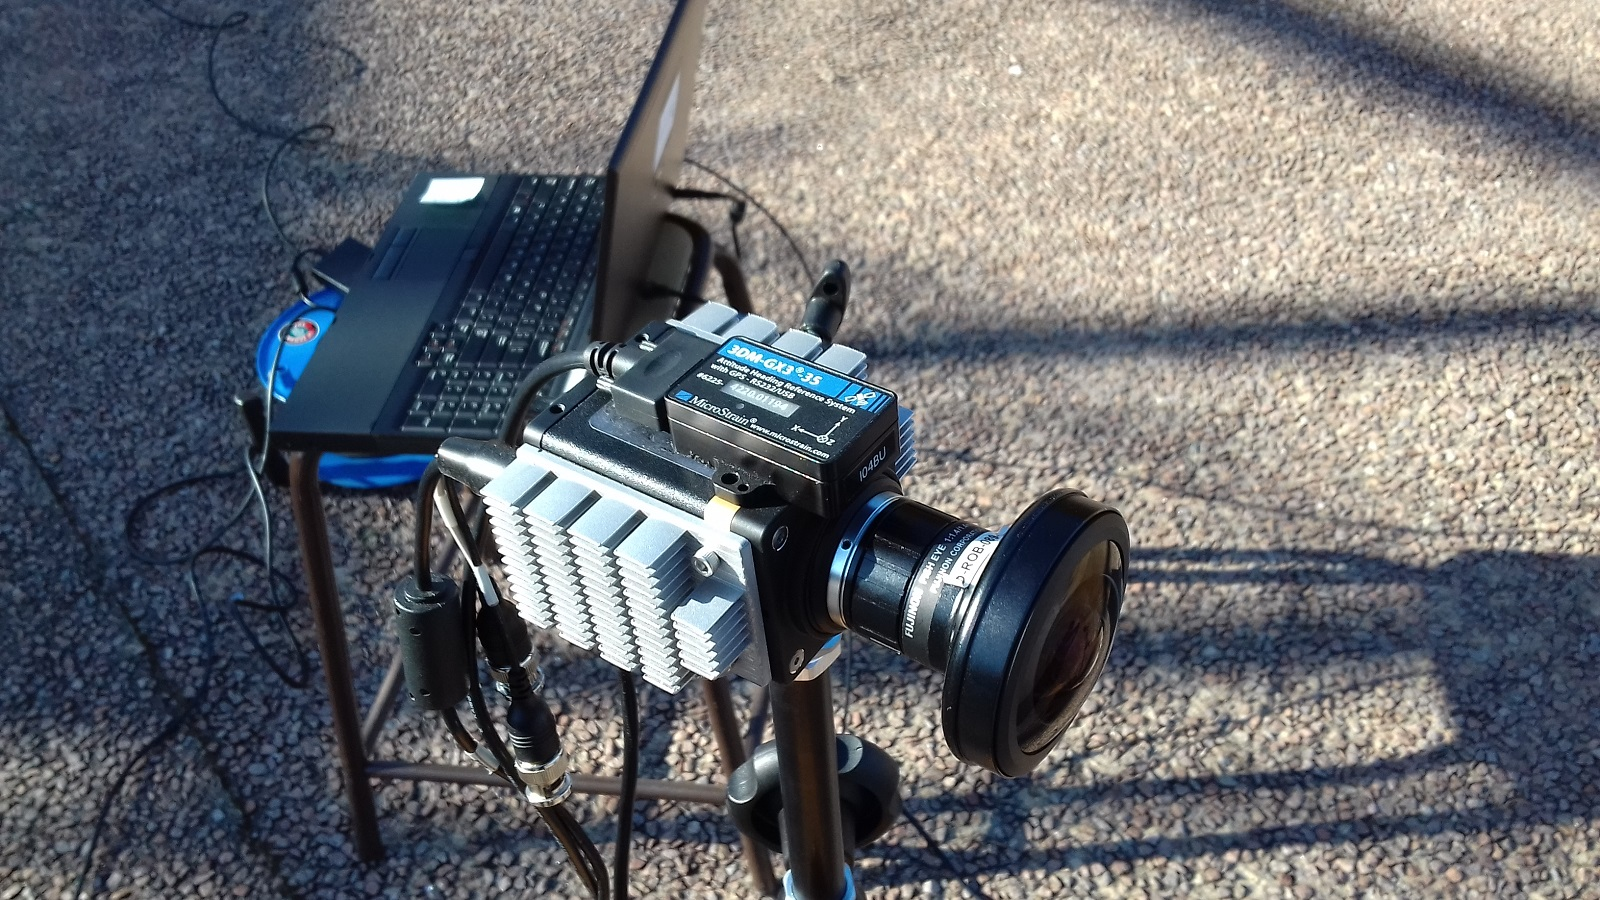
\includegraphics[width=0.33\textwidth]{./content/experiments/figures/setup.jpg}
\caption{The setup used for acquiring presented datasets in this paper}
\label{fig:setup}
\end{figure}
To be able to use the \gls{imu} recordings as \gls{gt}, this device
was calibrated with the camera using kalibr toolbox~\cite{furgale2013unified,
  furgale2012continuous}. The polarimetric camera with fisheye lens was also
calibrated according to~\cite{kannala2006generic}.

Using the above setup two data sets of synthetic and real images were created
and the results obtained are presented in Exp.~\ref{sec:exp1} and
Exp.~\ref{sec:exp2}, respectively.


\subsection{Experiment~1}
\label{sec:exp1}
The synthetic data containing \gls{aop} and \gls{dopl} images of sky regions
were created using the \gls{imu} recordings obtained during real acquisition.
Figure~\ref{fig:aop-dop-syn} shows an example of this dataset at
optimal conditions.
\begin{figure}
    \centering
    \subfigure[\gls{aop}]{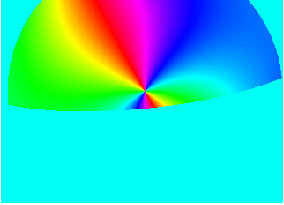
\includegraphics[width= 0.22\textwidth, height=0.12
      \textheight]{./content/experiments/figures/aop-no-noise.jpg}}\hfill
    \label{fig:aop-syn}
    \subfigure[\gls{dopl}]{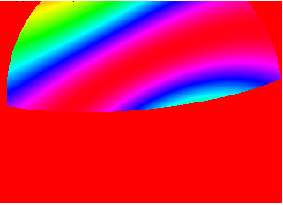
\includegraphics[width=0.22\textwidth, height=0.12
      \textheight]{./content/experiments/figures/dop-no-noise.jpg}}
    \label{fig:dop-syn}
    \hspace*{\fill}
    \caption{Synthetically created \gls{aop} and \gls{dopl} images of sky
      region for yaw, pitch and roll angle of 1.8, -0.2 and 0.1, respectively.}
    \label{fig:aop-dop-syn}
\end{figure}

Applying our framework on ideal synthetic data, perfect results were obtained
for absolute and relative rotations, while $\gamma$ was estimated using only
two random points from sky region (see Fig.~\ref{fig:res-syn-ideal-abs-rel}).
The synthetic dataset created based on \gls{imu} recordings, has rotation of
roll, pitch and yaw, respectively. This dataset has 856 samples, however for
simplicity, it has being down sampled by sampling rate of 30 samples.

\begin{figure}
  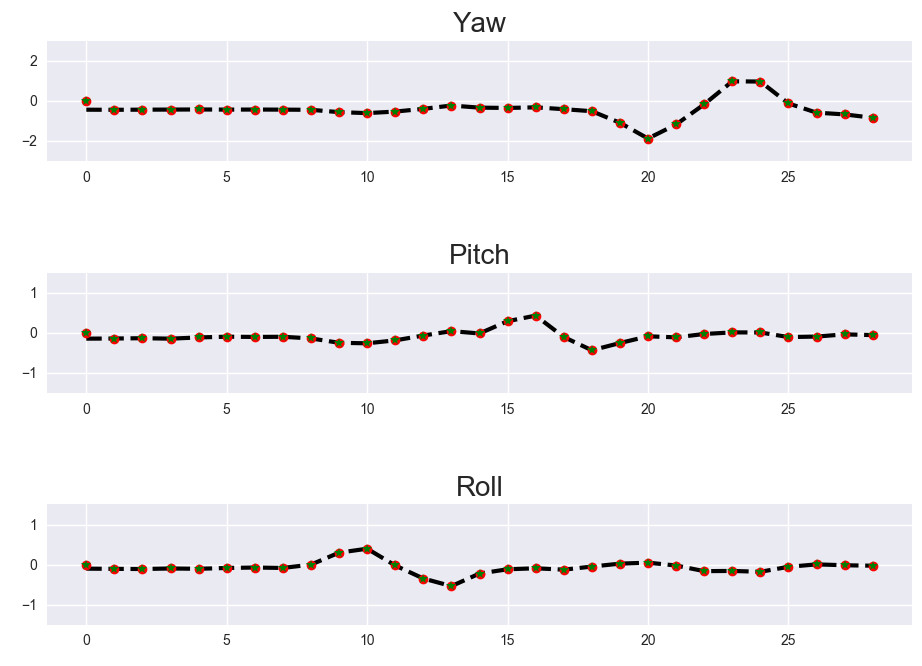
\includegraphics[width=0.47\textwidth]{./content/experiments/figures/ideal-syn-abs-rel-2.jpg}
  \caption{Absolute and relative rotation obtained from synthetic data in
    optimal conditions. The black line represents the \gls{gt}, the
    \textcolor{red}{dots} and the \textcolor{green}{stars} represent the
    absolute and relative predicted rotations, respectively.}
  \label{fig:res-syn-ideal-abs-rel}
\end{figure}

Although using our proposed framework we were able to achieve perfect results
on ideal synthetic data, in reality it is rare to obtain the perfect skylight
polarization pattern. Variety of causes clutter the desired skylight pattern,
main one being pollution. To account for such cases, a second test was
performed while significant level of noise was added to the created synthetic
data.
Figure~\ref{fig:aop-dop-syn-noisy} shows the an example of synthetic data with
$\%10$ noise.

\begin{figure}
  \centering
  \subfigure[\gls{aop}]{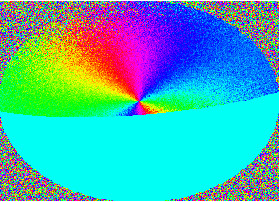
\includegraphics[width=0.22\textwidth,
    height=0.12\textheight]{./content/experiments/figures/aop-noise-01-2.jpg}
    \label{fig:aop-noise-syn}}\hfill
  \subfigure[\gls{dopl}]{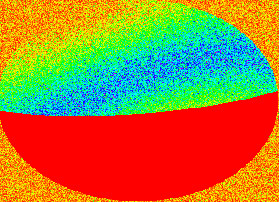
\includegraphics[width=0.22\textwidth,
    height=0.12\textheight]{./content/experiments/figures/dop-noise-01-2.jpg}
    \label{fig:dop-noise-syn}}
  \hspace*{\fill}
  \caption{Synthetically created \gls{aop} and \gls{dopl} images of sky
      region with noise level of $0.1$. With yaw, pitch and roll angle of 1.8, -0.2 and 0.1, respectively.}
  \label{fig:aop-dop-syn-noisy}
\end{figure}

Performing the same 2-random-point algorithm as before on noisy dataset leads
to the results illustrated in Fig.~\ref{fig:res-noisy-syn-abs-rel}. As expected the
performance decline, simply due to the noise.
% \begin{figure}
%   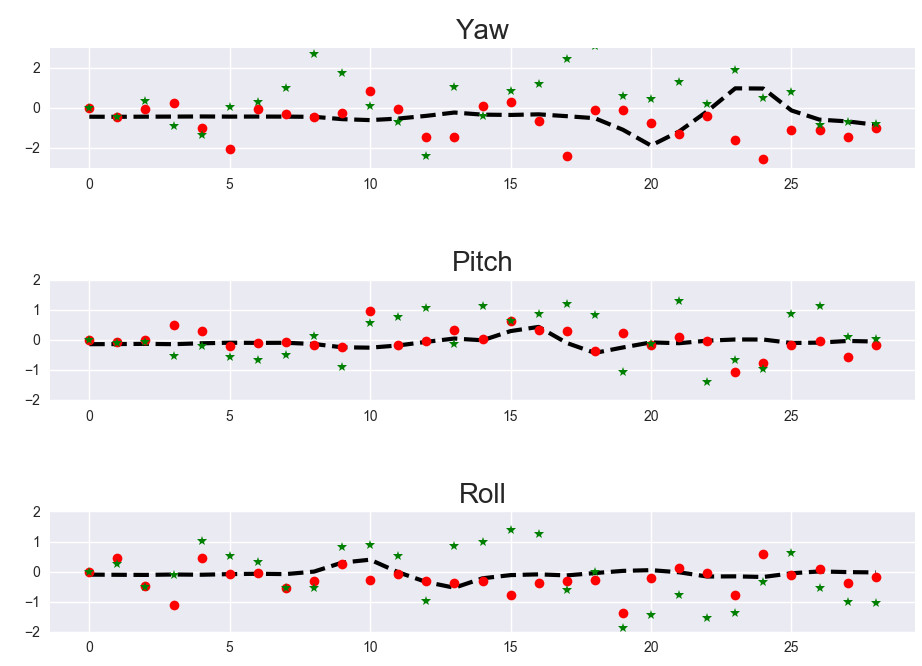
\includegraphics[width=0.5\textwidth]{./content/experiments/figures/noisy-syn-abs-rel-2.jpg}
%   \caption{Absolute and relative rotation obtained from synthetic data with
%     $10\%$ noise. The black line represents the \gls{gt}, the
%     \textcolor{red}{dots} and the \textcolor{green}{stars} represent the
%     absolute and relative predicted rotations, respectively.}
%   \label{fig:res-noisy-syn-abs-rel}
% \end{figure}

To solve this problem, two ransac models were defined for the absolute and
relative rotation, respectively.  In the proposed ransac model for absolute
rotation, since the sun position is assumed to be known the ransac model
optimizes the full rotation of each frame in comparison to the origin
considering the difference between the predicted and real sun positions.

The relative model, however, there is no information about the original
position, or sun position, and the algorithm only depends on the polarized
vector, $v = R_{cp}*v_p$ between two different frames. Therefore using the ransac
model, the optimal vector representing each frame is obtained.

Running our ransac models on the noisy datasets, with error threshold of 0.07,
10 random points (2 points for defining the model and the rest as test), and
2000 iterations the following results are obtained:
\begin{figure*}
  \centering
  \subfigure[The theoretical method without ransac optimization]{
    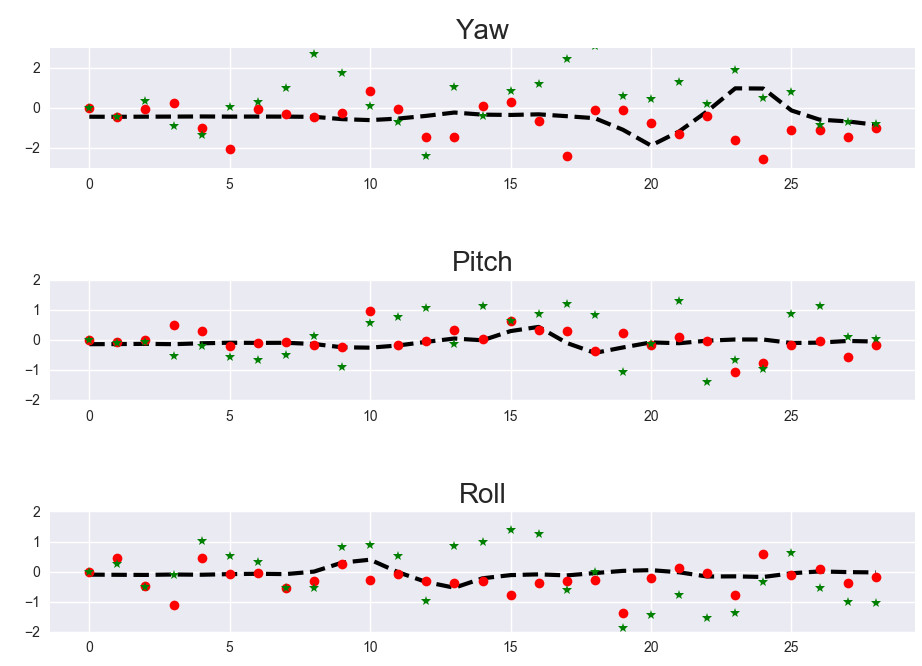
\includegraphics[width=0.47\textwidth]{./content/experiments/figures/noisy-syn-abs-rel-2.jpg}
  \label{fig:res-noisy-syn-abs-rel}}\hfill
  \subfigure[The theoretical method with ransac optimization]{
    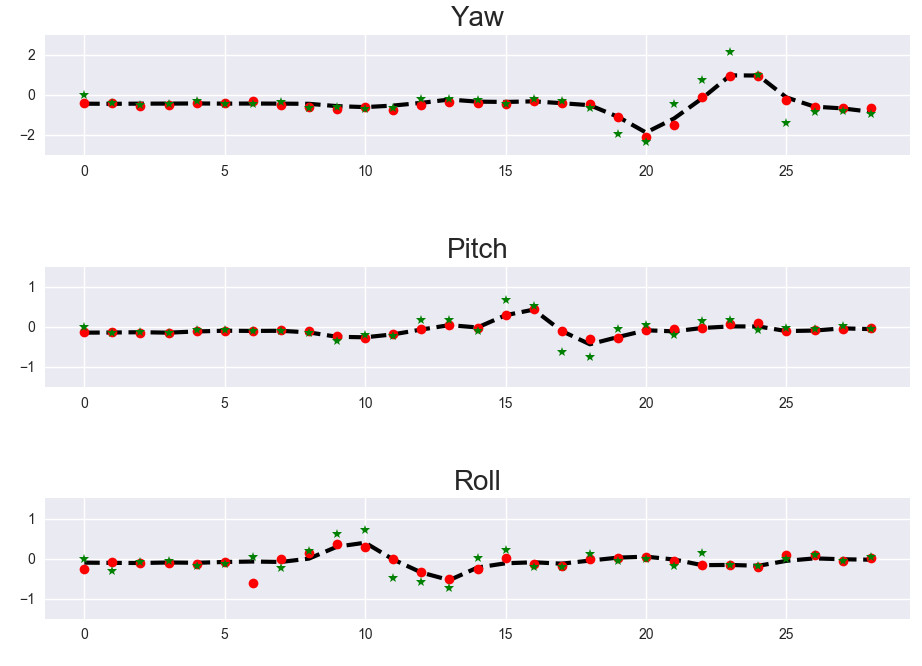
\includegraphics[width=0.47\textwidth]{./content/experiments/figures/noisy-ransac-abs-rel-3.jpg}
    \label{fig:res-noisy-syn-ransac-abs-rel}}
  \hspace*{\fill}
  \caption{Absolute and relative rotation obtained from  noisy synthetic data
    without and with ransac optimization. The black line represents the \gls{gt}, the
    \textcolor{red}{dots} and the \textcolor{green}{stars} represent the
    absolute and relative predicted rotations, respectively.}
  \label{fig:noisy-data}
\end{figure*}

The quantitative results in terms of mean difference ($\mu$) and standard
deviation ($\sigma$)
between the predicted rotations and \gls{gt} are tabulated in
Table.~\ref{tab:tab1}.

\begin{table}
  \centering
  \caption{Mean difference and standard deviation comparison between predicted
    results and \gls{gt} in radian.}
  \begin{tabular}{l cc cc cc}
    \toprule
    & \multicolumn{2}{c}{Yaw} & \multicolumn{2}{c}{Pitch} &
                                                            \multicolumn{2}{c}{Roll}\\
    \midrule
    & $\mu$ & $\pm \sigma$ &  $\mu$ & $\pm \sigma$ &  $\mu$ & $\pm \sigma$\\
    \cmidrule{2-3} \cmidrule{4-5} \cmidrule{6-7}

    Absolute & 0.087 & 0.078 & 0.020 & 0.029 & 0.068 & 0.100 \\
    Relative & 0.275 & 0.35 & 0.113 & 0.123 & 0.148 & 0.111\\
    \bottomrule
  \end{tabular}
  \label{tab:tab1}
\end{table}

As illustrated in the obtained results, using the ransac
model the outliers are ignored and satisfactory results are achieved.

\subsection{Experiment~2}
\label{sec:exp2}
This section presents the results obtained using real data. Same as previous
experiment the \gls{imu} results were used to create the \gls{gt} for vehicle
pose in the world frame.
The original data set contains 593 recordings. However for simplicity it was
down sampled with sampling rate of 20 frames.
Running ransac optimization with the same criteria as previous experiment the
following results are obtained (see Fig.~\ref{fig:res-real-ransac-abs-rel} $\&$
Table.~\ref{tab:tab2}).
\begin{figure}
  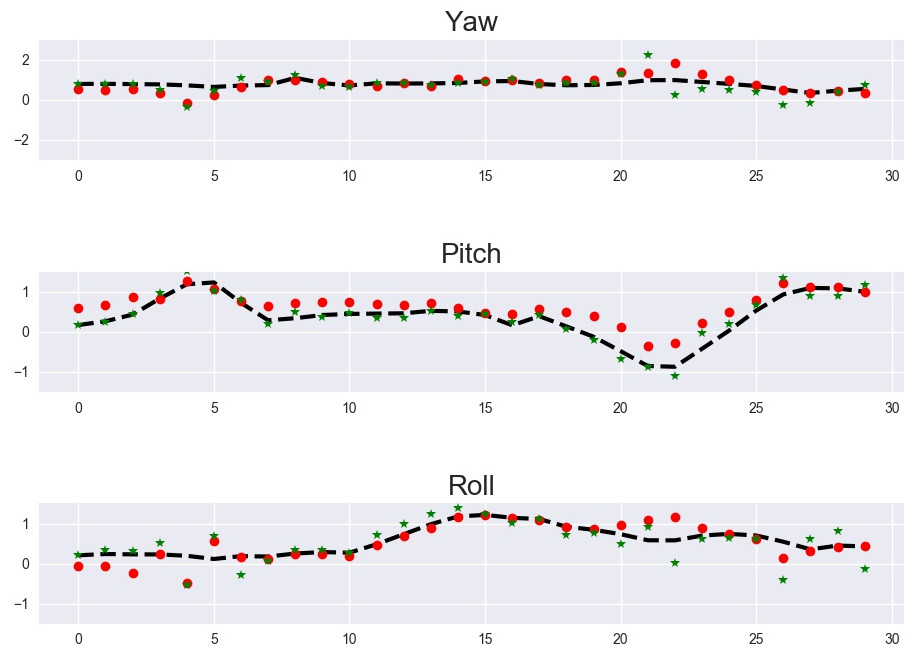
\includegraphics[width=0.47\textwidth]{./content/experiments/figures/real-ransac-abs-rel-2.jpg}
  \caption{Absolute and relative rotation obtained from real data. The black
    line represents the \gls{gt}, the \textcolor{red}{dots} and the
    \textcolor{green}{stars} represent the absolute and relative predicted
    rotations, respectively.}
  \label{fig:res-real-ransac-abs-rel}
\end{figure}


\begin{table}
  \centering
  \caption{Mean difference and standard deviation comparison between predicted
    results and \gls{gt} in radian on real data.}
  \begin{tabular}{l cc cc cc}
    \toprule
    & \multicolumn{2}{c}{Yaw} & \multicolumn{2}{c}{Pitch} &
                                                            \multicolumn{2}{c}{Roll}\\
    \midrule
    & $\mu$ & $\pm \sigma$ &  $\mu$ & $\pm \sigma$ &  $\mu$ & $\pm \sigma$\\
    \cmidrule{2-3} \cmidrule{4-5} \cmidrule{6-7}

    Absolute & 0.23 & 0.22 & 0.27 & 0.18 & 0.18 & 0.19 \\
    Relative & 0.37 & 0.40 & 0.20 & 0.18 & 0.20 & 0.18\\
    \bottomrule
  \end{tabular}
  \label{tab:tab2}
\end{table}


% Fig.~\ref{fig:res-syn-optimal}.
% \begin{figure}
%   \includegraphics[]{}
%   \caption{}
%   \label{}
% \end{figure}








%%%Local Variables:
%%% mode: latex
%%% TeX-master: t
%%% End:
